\chapter{Uczenie ze wzmocnieniem}
\label{cha:rozdzial3}

Przez wiele lat, wszelkie problemy optymalizacji były rozwiązywane przez 
określenie funkcji kosztu, która może być wielokryterialna, tzn. wiele 
zmiennych są optymalizowane. Często takie problemy są bardzo skomplikowane do 
rozwiązania analitycznego a czasem nawet niemożliwe. Często problemem jest 
wiele wymiarów, które składają się na problem optymalizacji. Dodatkowo zmienne 
stanu wpływają na siebie, a tym samym nie ma możliwości na optymalizację 
każdego parametru osobno.

Sama dziedzina uczenia ze wzmocnieniem jest uznawana, obok uczenia 
nienadzorowanego i uczenia nadzorowanego, za trzecią gałąź sztucznej 
inteligencji. Początki uczenia ze wzmocnieniem się dzielą na trzy oddzielne 
wątki, które przez wiele lat ewoluowały oddzielnie, aby pod koniec lat 80.-tych 
XX wieku połączyć się w uczenie ze wzmocnieniem jakie jest znane dzisiaj.

Pierwszy wątek opiera się na metodzie "prób i błędów" i wywodzi się z 
psychologii i badaniami nad zwierzętami. Drugi wątek traktował o sterowaniu 
optymalnym i rozwiązań stosujących funkcje kosztów i dynamicznego 
programowanie, które jest bardzo ważnym elementem uczenia ze wzmocnieniem, ale 
także rozwiązywanie problemów optymalizacji.

Mniej znaną gałęzią rozwijaną były badania związane nad uczeniem 
\textit{temporal -- difference}, które polega na porównywaniu wartości funkcji 
kosztów dla dwóch różnych chwil czasowych. 

Z biegiem czasu pojawiał się coraz mocniejszy sprzęt komputerowy, który 
umożliwiał uruchamianie bardziej zaawansowanych i rozbudowanych algorytmów. 
Dużą popularność uzyskał algorytm \textit{AlphaZero} opracowany przez firmę 
DeepMind w roku 2017, który przez mechanizm grania ze sobą (ang. \textit{self 
play}) i przeszukiwanie bardzo dużej przestrzeni stanów stosując heurystykę 
\textit{Monte -- Carlo Tree Search} był w stanie opanować gry t.j. szachy, 
shogi czy go i pokonać światowej sławy graczy. Szczególnie imponujące było 
bardzo szybkie opanowanie gry go, którą przez wiele lat uważano za niemożliwą 
do opanowania, ze względu na ogromną ilość możliwych pozycji, która została 
oszacowana na $2.1 \cdot 10^{170}$. 

Kolejnym bardzo dużym postępem w aktualnych badaniach związanych z uczeniem ze 
wzmocnieniem była kolejna iteracja AlphaZero od firmy DeepMind, \textit{MuZero} 
\cite{mu_zero}. Algorytm także stosował metody przeszukiwania Monte -- Carlo 
Tree Search do stworzenia ogólnego modelu, który był w stanie grać na 57 grach 
Atari. Nie znając wcześniej reguł powyższych gier, MuZero było w stanie 
osiągnąć wyniki przewyższające te osiągane przez człowieka. 

Do nauczenia powyższych algorytmów uczenia ze wzmocnieniem potrzebna było 
środowisko symulacyjne, wysokiej jakości sprzęt. Przeprowadzono wiele milionów 
iteracji, w których algorytm poprzez grę z samym sobą (termin w literaturze 
anglojęzycznej opisujący to podejście to \textit{self play}). Obiecujące jest 
to, że MuZero był w stanie opanować wiele gier różnych od siebie i o innych 
regułach w stopniu, który człowiekowi zająłby wiele lat.

\section{Podstawowe określenia i terminologia}

Zanim zostaną przedstawione najbardziej znane algorytmy uczenia ze 
wzmocnieniem, należy wprowadzić kilka podstawowych określeń i oznaczeń 
stosowanych w opinie problemów związanych z algorytmami uczenia ze wzmocnieniem.

\subsection{Agent i środowisko}

Głównymi elementami każdego algorytmu uczenia ze wzmocnieniem jest 
\textbf{agent} i \textbf{środowisko}, na który ten agent może wpływać. Bardzo 
często każdą symulację dzieli się na krótkie chwile czasowe, w których agent 
wykonuje jakąś akcję. Odnosząc to do naszego agenta, którym jest robot mobilny, 
taką akcją może być żądana prędkość liniowa i prędkość kątowa robota 
nieholomicznego. Zakładając, że środowisko jest choć częściowo obserwowalne, 
agent otrzymuje aktualny \textbf{stan środowiska} oraz \textbf{nagrodę}, która 
określa czy dana akcja zmieniała stan symulacji. Cały ten 
mechanizm został przedstawiony na rysunku \ref{fig:rlschematagentsrodowisko}.

\begin{figure}[H]
	\centering
	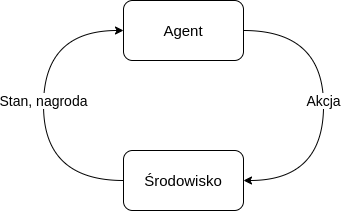
\includegraphics[width=0.5\linewidth]{rozdzial3/images/rl_schemat_agent_srodowisko}
	\caption{Schemat interakcji agenta ze środowiskiem. Źródło: opracowanie 
	własne}
	\label{fig:rlschematagentsrodowisko}
\end{figure}

Oznaczenia jakie się przyjmuje w literaturze:

\begin{itemize}
	\item $a_{t}$ -- akcja w chwili czasu $t$,
	\item $s_{t}$ -- stan (a dokładniej obserwacja) po wykonaniu akcji,
	\item $r_{t}$ -- nagroda, jaką agent otrzymał dla wykonanej akcji.
\end{itemize}

Głównym celem każdego algorytmu uczenia ze wzmocnieniem jest maksymalizacja 
skumulowanej nagrody. W trakcie nauki, agent może otrzymywać czasem wysokie 
nagrody w danej epoce, a czasem nawet utracić część nagrody, ale jeżeli 
skumulowana wartość rośnie, oznacza to, że agent zwiększa wiedzę na temat 
środowiska w jakim operuje.

\subsection{Przestrzenie akcji}

Różne algorytmy wymagają innych typów akcji. Wiele gier wirtualnych jak Atari 
czy Go ma wielowymiarowe przestrzenie akcji, które są \textbf{dyskretne}. 
Oznacza to, że liczba możliwych akcji, które agent może wykonać jest skończona. 
Przykładowo dla robota mobilnego takimi akcjami są: włącz silnik, wyłącz 
silnik, obróć się w lewo i obróć się w prawo. Niestety takie akcje dla wielu 
problemów nie mają zastosowania w praktyce. Dlatego kolejnym typem jest 
\textbf{przestrzeń ciągłych akcji}. Często te przestrzenie opisuje się wektorem 
liczb rzeczywistych. Przykładowo dla robota mobilnego taką akcją może być 
liczba rzeczywista z przedziału od 0 do 1, która opisuje wartość sterowania 
silnikiem, która przenosi się na wartość napięcia na silniku prądu stałego dla 
wartości od 0 wolt to 12 wolt.

\subsection{Polityki}

Każdy agent algorytmów uczenia ze wzmocnieniem podejmuje decyzję aby 
zmaksymalizować skumulowaną nagrodę. Jednak potrzebne są pewne reguły, jakimi 
taki agent będzie się kierował w trakcie eksploracji środowiska. Tak określana 
jest \textbf{polityka}, z którą agent podejmuje decyzje. W nomenklaturze 
oznacza się tą politykę grecką literą $\mu$. Polityki dzieli się na 
deterministyczne \ref{eq:deterministic_policy}:

\begin{equation}
	\label{eq:deterministic_policy}
	a_{t}=\mu(s_{t})
\end{equation}

Oznacza to, że akcja jaką wykona agent jest determinowana przez politykę tylko 
na podstawie aktualnego stanu środowiska, z którym agent wchodzi w interakcję.

Polityki mogą być także stochastyczne, czyli takie dla którym nie ma na sztywno 
zdefiniowanych akcji, dla konkretnych stanów środowiska. Akcja jest wybierana z 
pewnego rozkładu, na którym polityka (czyli agent podejmujący decyzję), zgodnie 
z równaniem \ref{eq:stochastic_policy}:

\begin{equation}
	\label{eq:stochastic_policy}
	a_{t}\sim\pi(\cdot|s_{t})
\end{equation}
 
Bardzo ważną dziedziną, która od momentu rozwoju wydajności sprzętu, jest 
głębokie uczenie ze wzmocnieniem \textit{deep reinforcement learning}. Jak 
nazwa sugeruje, w głębokim uczeniu ze wzmocnieniem korzysta się z sieci 
neuronowych, a wartości jej parametrów są optymalizowane korzystając z 
algorytmu optymalizacji. Dla sieci neuronowych najczęściej jest to algorytm 
gradientu najszybszego spadku. Dla rozwiązywania problemów głębokiego uczenia 
ze wzmocnieniem stosuje się sparametryzowane polityki, w których parametry 
oznacza się literą $\theta$. W literaturze często określa się równanie polityki 
jako \ref{eq:deep_rl}:

\begin{equation}
	\begin{aligned}
		\label{eq:deep_rl}
		a_t&=\mu_\theta(s_t)\\
		a_t&\sim\pi_\theta(\cdot|s_t)
	\end{aligned}
\end{equation}
 
\subsection{Trajektorie}
  
Kolejnym elementem uczenia ze wzmocnieniem są tzw. \textit{trajektorie}. 
Przyjmuje się, że jest to sekwencja stanów (używane zamiennie z obserwacjami) i 
akcji oznaczaną:

\begin{equation}
	\tau=(s_0, a_0, s_1, a_1,\dots)
\end{equation}

Przejścia między stanami, określane jako tranzycje, w chwili czasu $t$ oraz 
chwilą $t+1$, są tylko zależne od reguł danego środowiska oraz akcji, która 
została wykonana w chwili czasu $t$. Tak jak i z politykami mogą być one 
deterministyczne:

\begin{equation}
	s_{t+1}=f(s_t, a_t)
\end{equation}

lub stochastyczne:

\begin{equation}
	s_{t+1}=P(\cdot|s_t, a_t)
\end{equation}

Akcja $a_t$ jest wybierana zgodnie z polityką zastosowaną w danym algorytmie 
uczenia ze wzmocnieniem. Zwykle trajektoriami nazywa się \textbf{epizody}.

\subsection{Nagroda i zwrot}

Jednym z najważniejszych elementów uczenia ze wzmocnieniem jest funkcja nagrody 
\textit{R}. Zawsze zależy ona od 3 części, które składają się na opis całego 
środowiska do eksperymentu: aktualny stan świata (symulacji), aktualnej akcji 
jaka została wykonana na danym świecie oraz stanu środowiska po wykonaniu tej 
akcji. Opisuję się tą zależność zgodnie z równaniem \ref{eq:rl_reward}:

\begin{equation}
	r_t=R(s_t, a_t, s_{t+1})
\end{equation}

Celem jakiegokolwiek agenta jest maksymalizacja w pewien sposób określonej 
kumulatywnej nagrody po całej trajektorii. Taką nagrodę określa się poprzez 
$R(\tau)$. 

Jednym typem nagrody jest \textbf{nieprzeceniony zwrot o horyzoncie czasowym 
skończonym} (ang. \textit{finite -- horizon undiscounted reward}) określana 
przez \ref{eq:finite_horizon_undiscount_reward}:

\begin{equation}
	R(\tau)=\sum_{t=0}^{T} r_t
	\label{eq:finite_horizon_undiscount_reward}
\end{equation}	

Innym typem obliczanie skumulowanej nagrody jest zwrot z przeceną o 
nieskończonym horyzoncie czasowym (ang. \textit{infinite -- horizon discounted 
return}). Ta suma różni się od poprzedniej tym, że każda kolejna nagroda w 
przyszłości jest mnożona przez współczynnik zmniejszający się im dalej w 
przyszłości dana nagroda jest przyznawana. Współczynnik ten oznaczany jest 
przez $\gamma\in(0, 1)$. Równanie opisujące tą nagrodę 
\ref{eq:infinite_horizon_discount_reward}:

\begin{equation}
	R(\tau)=\sum_{t=0}^{\inf} \gamma^tr_t
	\label{eq:infinite_horizon_discount_reward}
\end{equation}	

Dlaczego stosowany jest głównie wzór \ref{eq:infinite_horizon_discount_reward}. 
Wynika to głównie ze stabilności i zbieżności takiej sumy do jakiejś wartości 
gdy czas zbiega to nieskończoności. Istotne jest to z powodu prostszego 
stosowania takiej sumy we wszelkich równaniach. Z kolei intuicyjnie odnosząc to 
równanie do dnia codziennego. Lepiej mieć teraz pieniądze niż jutro. Można 
dyskutować czy takie podejście do pieniędzy jest rozsądne (przykład: 
inwestowanie czy odkładanie pieniędzy na lokacie, które po wielu latach mają 
dają zwrot).

\subsection{Funkcje wartości}

W większości algorytmów uczenia za wzmocnieniem potrzebna jest informacja na 
temat \textbf{wartości} stanu lub pary stan -- akcja. Wartością określa się 
\textbf{oczekiwany zwrot} (ang. \textit{expected return}), która określa, że 
zaczynając ze stanu początkowego $s_0$ jakiej nagrody może oczekiwać agent 
zaczynając właśnie z tego stanu początkowego. Dlatego funkcje wartości w 
różnych formach są stosowane w wielu algorytmach uczenia ze wzmocnieniem, 
ponieważ umożliwiają określać czy dany stan będzie maksymalizował skumulowaną 
nagrodę, a tym samym poprawiał skuteczność agenta w danym problemie.

Funkcje wartości dzieli się na cztery główne typy:

\begin{enumerate}
	\item on -- policy value function,
	\item on -- policy action -- value function,
	\item optimal value function,
	\item optimal action -- value function. 
\end{enumerate}



